\chapter{4CP, Demand Response, and the Programs Beyond Price}
\chaptermark{4CP and Demand Response}
\label{ch:fourcp}

Every dollar in the last two chapters was set by a market: a settlement point price, a clearing price for readiness. This chapter is about the money that no market sets. Texas recovers the entire cost of its transmission grid, more than five billion dollars a year, through a rule that looks at one quarter-hour of each summer month and bills the utilities, and through them their largest customers, by how much each was consuming at that moment. % src: puct2025docket57491matrix (TCOS $5,446,864,795); puct25192(b)(1) (each DSP billed on its own 4CP demand); oncor2026retailtariff Rider TCRF (billing determinant kWh, NCP kW or 4CP kW by class) and secs. 6.1.1.1.3, 6.1.1.1.5, 6.1.1.1.6 (4CP kW for a premises that has set an NCP of 700 kW or more), 6.1.1.1.7 (Transmission Service, 4CP kW)
The rule is a tariff, an accounting convention adopted when the grid was a fraction of its present size, and it has become the single strongest reason a flexible load in Texas pauses. The grid operator and the market monitor both say so, and the Texas Legislature has now ordered the commission to re-examine it and amend its rules. % src: ercotboard2026dr (4CP drives most demand response in ERCOT); potomac2024som p. xxvii; texas2025sb6 sec. 6(a)(1) (evaluate "whether the current four coincident peak methodology ... ensures that all loads appropriately contribute"), 6(c) (amend commission rules by December 31, 2026 "to ensure that wholesale transmission charges appropriately assign costs for transmission investment"; no method prescribed)
This chapter explains the rule, shows when the four peaks actually landed and how hard they are to predict, prices the game, and then walks through the reform the commission has proposed to change it, along with the emergency programs that pay a load to respond when called.

\section{One Hour a Year}
\label{sec:fourcp-rule}

The rule is called 4CP, for Four Coincident Peak, which Chapter~3 introduced, and it works in two steps. % src: puct25192
First, every transmission owner in ERCOT divides its approved annual cost of service by the ERCOT-wide average of four numbers: the system's demand in the single 15-minute interval of highest demand in each of June, July, August, and September. % src: puct25192(b)(1); ercot2026protocols sec. 9.17.1(2)-(3)
The result is a rate in dollars per kilowatt of peak, and because every transmission owner charges the same way, their rates add up to one ERCOT-wide number that the Public Utility Commission calls the \glossaryterm{postage-stamp-rate}{postage stamp rate}: the same price for a kilowatt of peak demand anywhere in the state. Each utility's rate is set from its own filed cost of service and its own billing determinants, so the stamp is the sum of those rates rather than the state's total cost divided by the state's 4CP, and it lands about 2~percent above that quotient. % src: puct2025docket57491matrix ("Total ERCOT Postage Stamp Rate"); $5,446,864,795 / 81,042,657 kW = $67.21 against the posted $68.55, a 2.0% gap, and the 2013 pair divides out the same way ($30.32 against $30.95); puct2013docket40946matrix, footnote to the TOTAL row: the sum of the approved TCOS "will not match the postage stamp rate multiplied by 2012 ERCOT Average 4CP because the TCOS for most TSPs was approved under the ERCOT 4CP from prior years"; analysis/checks/ch8_postage_stamp.py
Second, the wires utility that delivers power to your site, the transmission and distribution utility of Chapter~6, pays that rate on its own customers' demand during those same four intervals and passes the bill down class by class: households and small shops pay their share by the kilowatt-hour, mid-sized sites by their own monthly peak, and only the largest, a transmission-voltage site among them, by the average of their own draw across those four intervals. % src: puct25192(b)(1),(d); puct25193; oncor2026retailtariff Rider TCRF (Sheet 6.1, Revision 52, effective August 1, 2026: charge = TCRF x "the Retail Customer's appropriate monthly billing determinant (kWh, 4 CP kW or NCP kW)", class shares by the last rate case's allocator; Residential and Secondary <= 10 kW per kWh, Secondary > 10 kW per NCP kW or 4CP kW, Transmission Service per 4CP kW), secs. 6.1.1.1.3, 6.1.1.1.5, 6.1.1.1.6 (a premises that has set an NCP of 700 kW or more is billed on 4CP kW, a smaller one on its monthly NCP kW), sec. 6.1.1.1.7 (Transmission Service, Determination of 4CP kW: "the average of the Retail Customer's integrated 15-minute demands at the time of the monthly ERCOT system 15-minute peak demand for the months of June, July, August and September of the previous calendar year", read 2026-09-27); centerpoint2026retailtariff, the same three tiers: Sheet 6.13, 53rd Revision, effective September 1, 2026 (Residential and Secondary <= 10 kVA per kWh, Non-IDR per NCP kVA, IDR and Transmission Service per 4CP kVA), Sheets 6.3-6.4 (IDR charges for a customer that has set an NCP "greater than 700 kVA")
If your site is one of them, your share of Texas's transmission bill for all of next year is set by your meter reading in four quarter-hours of this summer. Each quarter-hour carries a quarter of it: consume nothing in all four and the transmission charge on your bill goes to zero for twelve months, run at full draw through one and you pay a quarter. A new site is billed on an estimate until it has a summer of its own (Chapter~9). % src: puct25192(b)(1),(d) (the four intervals of the prior summer set the next year's charge); oncor2026retailtariff sec. 6.1.1.1.7 (the charge is on the average of the four, so one interval at full draw bills 1/4 of the annual charge); oncor2026retailtariff Sheet 1.7 (Revision Twelve, effective June 1, 2026) p. 2 (a)-(b): a Retail Customer without previous history is billed on estimated 4CP kW, the average of its actual CP kW if it has at least two and they are representative (otherwise an estimate by mutual agreement), NCP kW times the transmission class coincidence factor if it has fewer than two; centerpoint2026retailtariff Sheet 6.5 pp. 2-3, the same for 4CP kVA; chapter 9 sec:stack-rule step 5

The size of the prize has more than doubled in a decade. In 2013 the postage stamp rate was \$30.95 per kilowatt-year on a 4CP of 66~GW, recovering a \$2.0~billion cost of service. % src: puct2013docket40946matrix ($30.950950/kW-yr; 66,014,375.9 kW; $2,001,794,430)
For 2025 it was \$68.55 per kilowatt-year on a 4CP of 81~GW, recovering a \$5.4~billion cost of service: the rate up 121~percent, the cost up 172~percent, the peak up 23~percent. % src: puct2025docket57491matrix ($68.547301/kW-yr; 81,042,657 kW; $5,446,864,795, the filed TCOS: stamp x 4CP is $5.555 bn, the 2% gap of the line above); nrg2025comments58484 (121% since 2013); analysis/checks/ch8_postage_stamp.py (+121% rate, +172% TCOS, +23% 4CP)
Divide by four and each of the four intervals is worth about \$17,100 per megawatt at the wholesale level, and one energy executive, treating each interval as if it were an hour, calls 4CP ``a \$16,700 per megawatt-hour price signal,'' more than three times the energy market's price cap, delivered without the energy market's help \autocite{puct2025docket57491matrix,puct2013docket40946matrix,kavulla2025remarks}. % src: puct2025docket57491matrix ($68,547/MW-yr / 4 = $17,137 per interval); kavulla2025remarks ($16,700/MWh); HCAP $5,000/MWh per potomac2021som

What a site actually pays depends on its wires utility, because each utility passes the wholesale bill through a rider that is trued up twice a year and allocated by its own last rate case \autocite{puct25193}. % src: puct25193 (TCRF updated March 1 and September 1); oncor2026retailtariff Rider TCRF
Oncor, whose territory carries about 36~percent of ERCOT's peak, charges a transmission-connected customer \$3.49 per kilowatt of 4CP demand per month from August 2026, which is about \$41,900 per megawatt-year; the same rider stood at \$4.85 in September 2024, or about \$58,300. % src: puct2025docket57491matrix (Oncor 28,908,860.870 of 81,042,657 kW = 35.7%); oncor2026retailtariff Rider TCRF ($3.491759 eff. Aug 1, 2026 = $41,901/MW-yr; $4.854456 eff. Sept 1, 2024 = $58,253)
CenterPoint's Houston territory bills about \$5.05 per kilovolt-ampere (apparent power, close to a kilowatt for a site with good power factor) per month from September 2026, roughly \$60,600 per megavolt-ampere-year \autocite{centerpoint2026retailtariff}. % src: centerpoint2026retailtariff ($5.048210/kVA-mo x 12 = $60,578.52)
On the transmission-service riders in force from September 1, 2025, the four investor-owned utilities ranged from about \$40,700 per megawatt-year at Oncor, through \$55,700 at AEP Texas and \$61,900 at TNMP, to \$66,700 at CenterPoint, so a single 15-minute interval was worth \$10,000 to \$17,000 per megawatt of load that managed to be absent from it \autocite{oncor2026retailtariff,aep2025tcrf58157,tnmp2025tcrf58161,centerpoint2025tcrf58178}. % src: Transmission Service class TCRF effective 2025-09-01, x 12,000: oncor2026retailtariff Rider TCRF history row for 2025-09-01, $3.395215/4CP kW = $40,742.58/MW-yr (since raised to $3.491759 = $41,901); aep2025tcrf58157 $4.641723/avg 4CP kW = $55,700.68; tnmp2025tcrf58161 $5.156858/4CP kVA = $61,882.30; centerpoint2025tcrf58178 $5.557160/4CP kVA = $66,685.92 (per MVA; kVA taken as kW at good power factor, as above); /4 = $10,185.65 to $16,671.48 per interval
NRG's survey of the same tariffs, filed that month, put the top of the range at \$85,300, but that is TNMP's rider for commercial customers served at secondary, low voltage, not a rate a transmission-voltage mine pays \autocite{nrg2025comments58484}. % src: nrg2025comments58484 fn. 29 (Sept. 9, 2025 filing; floor = Oncor transmission class $3.395215 = $40,742.58/MW-yr; ceiling = TNMP secondary > 5 kW class $7.109469 = $85,313.63); tnmp2025tcrf58161 (Secondary Service Greater Than 5 KW, IDR Metered, $7.109469 per 4CP kW)
The Oncor access rate quoted in Chapter~6 was that one utility's own slice of the postage stamp; the bill a site sees is built from the whole stamp, split among customer classes in the utility's last rate case. That is why the retail figures above differ from the \$68,550 per megawatt-year wholesale rate: in September 2025 every transmission-voltage rider landed below it, while a lower-voltage one such as TNMP's secondary rider landed above. % src: oncor2025transmissiontariff (Oncor's Rate NTS $21,434.64/MW = 31% of the $68,547 postage stamp); transmission-class riders $40,743-$66,686 < $68,547 (sources above); TNMP secondary > 5 kW IDR $85,313.63 > $68,547 (tnmp2025tcrf58161)

Three details of the rule matter for anyone trying to beat it. The peak is measured on ERCOT's settlement data, not on the live demand number on ERCOT's dashboard; the settlement figure excludes the charging of grid batteries and power flowing out over the DC ties to neighboring grids, so the two can disagree about which quarter-hour was the peak. % src: ercot2026protocols sec. 9.17.1(3) (formula excludes DC-tie exports and Wholesale Storage Load; the NPRR1188 gray box, upon system implementation, also subtracts non-ALR CLR load and non-WSL charging load supplied by co-located generation at net-metered sites, and sec. 11.1.6(4)(c) keeps a CLR's grid-supplied load in its 4CP, see chapter 3 sec:4cp-intro); ercot2024mktnotice4cp
Section~\ref{sec:fourcp-peaks} shows how often they do. The peak is not known when it happens: settlement statements arrive five and fifty-five days after each operating day, so a June peak is not final until late August, and ERCOT files the year's official four intervals with the commission by December 1 for billing the following year \autocite{ercot2026protocols,ercot2024mktnotice4cp}. % src: ercot2026protocols secs. 9.5.4-9.5.5 (RTM Initial and Final Statements at 5 and 55 days), 9.17.1(1) (December 1); puct25192(d)
And there is no weekday rule and no holiday rule: any quarter-hour of any day in the four months can be the one.

\section{When the Peaks Land}
\label{sec:fourcp-peaks}

Table~\ref{tab:fourcp-official} lists every official ERCOT 4CP interval for eight summers, from ERCOT's own filings. % src: analysis/data/ercot_official_4cp_2018_2025.csv (ERCOT NP9-83-M workbooks 2022-2025; PUCT Project 51878 Item 52 for 2021; ERCOT 1996-2020 archive for 2018-2020, 2019 as revised)

\begin{table}[htbp]
  \centering
  \footnotesize
  \setlength{\tabcolsep}{3.5pt}
  \begin{tabular}{lllllr}
    \hline
    \textbf{Year} & \textbf{June} & \textbf{July} & \textbf{August} & \textbf{September} & \textbf{Avg GW} \\
    \hline
    2018 & 27th 17:00 & 19th 17:00 & 23rd 16:45 & 19th 16:30 & 69.4 \\
    2019 & 19th 17:00 & 30th 16:30 & 12th 17:00 & 6th 16:45 & 71.0 \\
    2020 & 8th 17:45 & 13th 16:45 & 13th 16:45 & 1st 14:30 & 70.5 \\
    2021 & 23rd 17:00 & 26th 17:00 & 24th 17:00 & 1st 17:00 & 72.5 \\
    2022 & 23rd 17:00 & 20th 16:45 & 2nd 17:00 & 20th 17:00 & 76.7 \\
    2023 & 27th 17:00 & 31st 17:00 & 10th 17:00 & 8th 16:45 & 83.6 \\
    2024 & 30th 17:45 (Sun) & 1st 17:00 & 20th 17:00 & 20th 16:00 & 81.0 \\
    2025 & 19th 17:00 & 30th 17:00 & 18th 17:00 & 4th 17:30 & 80.9 \\
    \hline
  \end{tabular}
  \caption{The official ERCOT 4CP intervals, 2018 to 2025: day of the month and ERCOT's label for the 15-minute settlement interval (Central prevailing time), with the year's average 4CP demand. The label names the interval's end, so the interval labeled 17:00 ran from 4:45 to 5 in the afternoon \autocite{ercot4cp2016puct}. The one weekend interval in eight years is marked. Sources: ERCOT's annual 4CP calculation workbooks (data product NP9-83-M) for 2022 to 2025, ERCOT's report to the commission for 2021, and ERCOT's 1996--2020 archive for 2018 to 2020 \autocite{ercotnp983m,ercot4cp2021puct,ercot4cphistzip}.} % src: analysis/data/ercot_official_4cp_2018_2025.csv (per-row provenance in the file); averages: 69,369.0 / 70,980.9 (revised) / 70,488.3 / 72,490.3 / 76,713.9 / 83,556.8 / 81,042.7 / 80,859.8 MW; label = interval end: ercot4cp2016puct p. 2 ("Interval Ending (IE) 16:00", the workbook's 7/14/2016 16:00), ercot4cphistzip (2006 filing workbook: "at interval ending 16:15" beside the bare 6/13/2006 16:15 header), ercot2026protocols sec. 10.9.1(2)(h); corroborated by the ch8_4cp_peaks.R convention check (27 of 28), read through analysis/checks/official_4cp.R
  \label{tab:fourcp-official}
\end{table}

Read down the time column and the first regularity jumps out. All 32 intervals ended between 2:30 and 5:45 in the afternoon, 30 of them inside a single 90-minute window, the six consecutive quarter-hours from 4:15 to 5:45, and 19 of them carry exactly the same label, 17:00, the quarter-hour that ends at 5~p.m. % src: analysis/checks/ch8_4cp_peaks.R console (32 official intervals, labels between 14:30 and 17:45; 30 labels in 16:30-17:45, i.e. intervals within 16:15-17:45 = six quarter-hours, 90 min; 19 labeled 17:00, the interval 16:45-17:00)
Thirty-one of thirty-two were weekdays; the exception was Sunday, June 30, 2024, when a heat wave on the last day of the month set a June peak no weekday had reached. % src: analysis/checks/ch8_4cp_peaks.R console (weekend: 1, 2024-06-30); analysis/data/ercot_official_4cp_2018_2025.csv
The dates are far less regular: June's peak has fallen anywhere from the 8th to the 30th, September's from the 1st to the 20th, and in 2024 the June and July peaks were a day apart across the month boundary. That combination, a predictable hour on an unpredictable day, is the shape of the whole forecasting problem. % src: analysis/data/ercot_official_4cp_2018_2025.csv (June 8th to 30th: 2020-06-08 and 2024-06-30; September 1st to 20th: 2020/2021-09-01 and 2022/2024-09-20; 2024-06-30 and 2024-07-01 adjacent)

\begin{figure}[htbp]
  \centering
  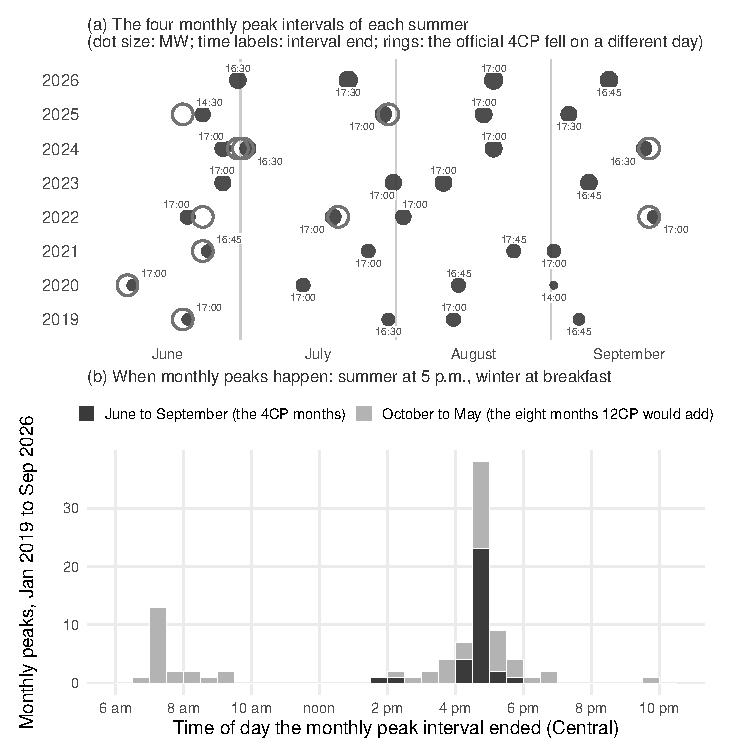
\includegraphics[width=\textwidth]{images/fourcp_calendar}
  \caption{
    (a)~The four monthly peak intervals of each summer since 2019, reconstructed from ERCOT fuel generation as a demand proxy; where ERCOT's official 4CP fell on a different day, a ring marks the official date. Dot size scales with megawatts. (b)~The time of day of every monthly peak from January 2019 to September 2026, the four 4CP months against the other eight: summer peaks cluster at 5~p.m., winter peaks cluster around 7:30~a.m. Generation is net of storage charging, with DC ties omitted and no gap-filling; the official 4CP dates are from ERCOT's annual 4CP workbooks. % fig-src: analysis/figures/fig_ch8_4cp_calendar.R on analysis/data/ercot_monthly_peak_intervals_reconstructed.csv (analysis/checks/ch8_4cp_peaks.R: ercot_fuel_mix_15min_2019on.csv.gz via ch8_demand.R, no gap-fill, complete months) and analysis/data/ercot_official_4cp_2018_2025.csv
  }
  \label{fig:fourcp-calendar}
\end{figure}

Figure~\ref{fig:fourcp-calendar}(a) rebuilds the peaks from ERCOT's Fuel Mix Report: generation summed across fuels, including the battery-charging adjustment, as a generation-based demand proxy \autocite{ercotfuelmixhistory}. It omits net imports over the DC ties and does not separately reconstruct \glossaryterm{block-load-transfer}{Block Load Transfers}: groups of customers disconnected from their usual grid area and connected to a neighboring one \autocite{ercot2026protocols}. In the reports for 2019 to 2021, the battery-charging adjustment sits inside ``Other''; from 2022 it has its own category. Summing all categories includes it in both periods. The proxy already nets out battery charging. Subtracting it again would count the adjustment twice. This is a settlement reconstruction, not a live feed; August and September 2026 are still initial settlement. It matches 17 of the 28 official peak dates in 2019 to 2025, so the official filings remain the authority on which afternoon won. % src: analysis/checks/ch8_4cp_peaks.R console (17 of 28 dates match; 24 of 28 daily peak intervals match the official label; 14 of 28 monthly peak intervals match); analysis/data/fetch_ercot_fuel_mix.py and ercot_fuel_mix_15min_2019on.csv.gz (2019-2021 Summary notes include WSL adjustments in Other; WSL separate from 2022; FINAL through July 2026, INITIAL August-September 2026); ercot2026protocols sec. 2 (Block Load Transfer definition) and sec. 9.17.1(3) for BLT terms; ercotfuelmixhistory

The accounting detail from Section~\ref{sec:fourcp-rule} matters even when watching ERCOT's own live demand number: battery charging counts there and not in the settlement peak. The exclusion dates to February 2013 \autocite{ercotnprr461}. ERCOT reminded participants of this in August 2024 and later confirmed that storage charging and DC-tie treatment moved the winning date in June and September 2024 \autocite{ercot2024mktnotice4cp,ercottwg20254cp}. % src: ercotnprr461 (Board Report 121112, sec. 9.17.1(3); effective 2013-02-14 for this section; independently checked against January 2019 Protocols sec. 9.17.1(3)); ercot2024mktnotice4cp (WSL included in operational load, excluded from settlement 4-CP); ercottwg20254cp (Deviation from Operation Load: WSL and DC-tie treatment, twice in 2024, June and September); these are ERCOT's operational-versus-settlement findings, not an attribution of the fuel-mix proxy's residual errors
A 4CP forecast has to model the settlement definition, batteries subtracted, or it will celebrate the wrong afternoon.

Two more patterns sit in the data. The peaks are climbing: the annual peak in this reconstruction rose from 74.1~GW in 2019 to 91.5~GW on August 20, 2026, the highest through September, and the lowest monthly peak of the year rose from 52~GW in 2019 to 62~GW in 2025. The proxy does not establish an official record: ERCOT's provisional demand record is about 91.2~GW on July 22, 2026 \autocite{ercot2026factsheet}. % src: analysis/checks/ch8_4cp_peaks.R console (2019 peak 74,075 MW; 2026 peak 91,455 MW on 2026-08-20 interval ending 17:00; lowest monthly peaks 52,130 MW in Apr 2019 to 62,392 MW in Dec 2025; 2026 nine complete months only; September 2026 peak 87,187 MW on 2026-09-12 interval ending 16:45, below August); ercot2026factsheet October 2026 edition read 2026-11-01 (91,155 MW on July 22, unofficial until final settlement; was 91,134 MW in the edition read 2026-09-27; mutable PDF)
And the summer peak hour is not moving, while the hour that matters to the grid is. Chapter~6 showed the net-load peak, demand minus wind and solar, sliding into the evening; ERCOT's own summer reviews put it at hour ending 21 (8 to 9~p.m.) in 2023 and 2024 and hour ending 22 in June and July 2025. % src: ercotsummer2025review (net load hour HE 21 -> HE 22); ch6 sec. 6.6 (IMM: tightest hours 7-9 p.m.)
The 4CP interval, which counts gross demand with solar still shining, has stayed at 5~p.m. all along. So the one hour Texas uses to allocate its transmission costs is no longer the hour the system is short of power; ERCOT told its board in 2026 that 4CP ``does not correspond to the system's highest net-load peaks,'' even as it remains the strongest load-reduction incentive in the state \autocite{ercotsummer2025review,ercotboard2026dr}. % src: ercotboard2026dr
Hold that thought for Section~\ref{sec:twelvecp}; I read it as one reason the commission has proposed to rewrite the rule.

\section{What Makes a Peak, and How Hard It Is to Call}
\label{sec:fourcp-factors}

Ask what sets a Texas summer peak and the first answer is weather: afternoon temperature across the big load centers drives air-conditioning, and air-conditioning drives the peak. Weather is necessary but not sufficient, because the peak is a competition between afternoons. A Tuesday at 104 degrees Fahrenheit (40 Celsius) sets the July peak only if no other July afternoon is hotter, or later in the month with more load connected, or less relieved by clouds over Houston. Five factors decide that competition.

The first is the calendar. Load grows within the summer as more equipment is energized, so late-month afternoons carry a structural edge; the table shows peaks clustering late in June and July. The second is the weekday, because the same temperature produces more demand on a workday than a Sunday, which is why 31 of 32 peaks were weekdays and the one Sunday needed a month-end heat wave to break the pattern. % src: analysis/checks/ch8_4cp_peaks.R console
The third is the hour, and here the grid does the forecaster a favor: the gross-demand peak lives at 5~p.m.\ because that is when air-conditioning demand and still-working offices overlap before solar fades, and Figure~\ref{fig:fourcp-calendar}(b) shows how tightly it clusters. The fourth is the settlement accounting just described, batteries and DC-tie flows netted out of the official number. And the fifth is the strangest: the peak is shaped by the people chasing it. ERCOT estimates that on August 18, 2025, the summer's peak day, cryptocurrency mines cut about 3,150~MW and identifiable 4CP response about 1,500~MW at the peak hour, so that the recorded peak of 83,878~MW would have been roughly 88,500~MW without those reductions. % src: ercotsummer2025review slide 10 (83,878 MW HE17; ~3,151 MW crypto reduction; ~1,501 MW 4CP reduction; 88,530 MW estimated without reductions)
Across the years ERCOT has put the load actively dodging 4CP intervals at as much as 4,000~MW in 2021, 3,500~MW in 2023, 2,500~MW in 2024, and 1,500~MW of 4CP response beyond the mining reduction in the August 2025 interval \autocite{ercotsummer2025review,potomac2021som,potomac2023som,potomac2024som,potomac2026somercot}. % src: potomac2021som p. 39; potomac2023som pp. 34-35; potomac2024som pp. 33-34; potomac2026somercot p. 31 (all relaying ERCOT estimates)
The chairman of the Public Utility Commission described the effect from his side of the table: ``you can actually see usage go down because they're chasing that interval'' \autocite{tep2026gleeson}. % src: tep2026gleeson (Gleeson interview, June 2026)
When several gigawatts of load vanish on the afternoons everyone expects to be the peak, the peak sometimes moves to an afternoon nobody expected. The forecast changes the thing it forecasts. Game theorists have started to formalize this. A 2025 preprint from Columbia University models coincident-peak avoidance as a game among flexible loads. It observes that the forecasting literature treats each load as a price-taker and ignores the effect of everyone's response on the peak being predicted. It finds that when the players are flexible enough the equilibrium is a flattened peak, with system demand pushed toward equality across the contested periods, at an efficiency cost that grows with the players' flexibility \autocite{chen2025cpgaming}. % src: chen2025cpgaming (arXiv 2501.02792v5: Sec. I on prediction studies neglecting agents' effect on CP predictions; Theorem 1 and Sec. VI: agents balance system demand across periods at equilibrium; Theorems 5-6: efficiency loss grows with flexibility and cost disparity)
The many near-equal afternoons of 2025 (Figure~\ref{fig:fourcp-window}) are consistent with that equilibrium, although a hot, flat summer could have produced them on its own.

\begin{figure}[htbp]
  \centering
  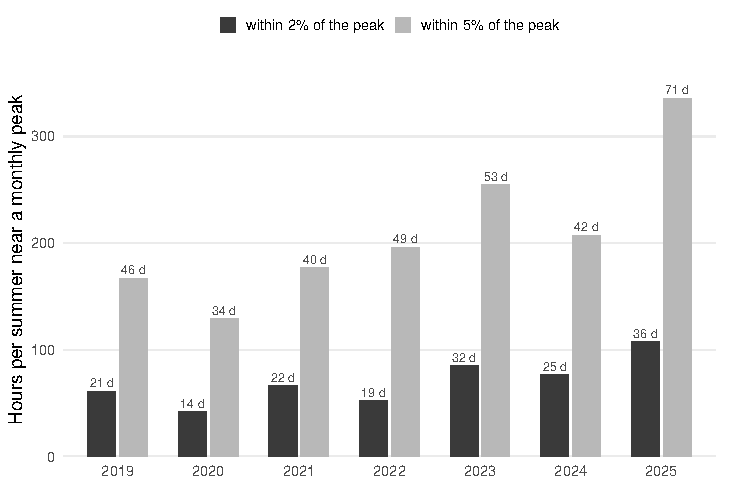
\includegraphics[width=\textwidth]{images/fourcp_window}
  \caption{
    The size of the haystack: hours per summer in which the demand proxy came within 2~percent and within 5~percent of that month's eventual peak, summed over June to September, with the number of distinct days those hours fell on. These are hindsight counts: they assume the height of each peak was known in advance, which in a running season it is not; Table~\ref{tab:fourcp-rules} scores the rules a site can actually run. % fig-src: analysis/figures/fig_ch8_4cp_window.R (summers pinned to 2019-2025) on analysis/data/ercot_fuel_mix_15min_2019on.csv.gz, checked by analysis/checks/ch8_demand.R, no gap-fill
  }
  \label{fig:fourcp-window}
\end{figure}

How hard is the call, then? Figure~\ref{fig:fourcp-window} measures the haystack in hindsight. In a typical summer, 66 hours of 15-minute intervals spread over 22 different days came within 2~percent of one of the four monthly peaks; loosen the tolerance to 5~percent and it is about 196 hours over 46 days. % src: fig_ch8_4cp_window.R console (within 2%: median 66.25 h, 22 days; within 5%: median 196.25 h, 46 days; generation-based proxy, no gap-fill)
2025 was the hardest year in the sample, with 108 hours within 2~percent over 36 days, because a hot, flat summer produced many afternoons of nearly equal height. % src: fig_ch8_4cp_window.R console (2025: 108 h, 36 days within 2%)
Those counts are floors, because they assume the site knew in advance how high the peak would be. In a running season nobody does: the line that defines ``within 2~percent'' is drawn only when the month is over and the tallest afternoon is known.

What a site can actually do without a forecast is run a rule on information it has, and Table~\ref{tab:fourcp-rules} scores four such rules against the 28 official intervals of 2019 to 2025. The clock rules need only the calendar; the demand rules are estimated retrospectively on the demand proxy, which was not available live. % src: analysis/checks/ch8_4cp_rules.R console
Pausing every afternoon from 2 to 6 catches every peak and costs about 490 hours a summer. Pausing weekdays from 4 to 6 costs about 175 hours and lets three of the 28 through: the Sunday peak of June 2024 and two quarter-hours that were over by the time the window opened, the one ending at 2:30 on September 1, 2020 and the one ending at 4:00 on September 20, 2024. % src: ch8_4cp_rules.R console (calendar arithmetic: rule A 488 h every summer, 28 of 28; rule B 172-176 h, median 174, 25 of 28; lets through 2020-09-01 14:15-14:30, 2024-06-30 17:30-17:45 Sunday, 2024-09-20 15:45-16:00)
A threshold on live demand, set against the previous summer's highest peak because that is the only height a site knows in advance, fails in both directions. In the record summers of 2022 and 2023, when June demand already exceeded the previous year's peak, the 95~percent rule idled the site for more than 400 hours. In the milder summers of 2019, 2024, and 2025 it paused about 70 to 75 hours yet caught only one or two of the four peaks, because a mild summer's peaks fall short of last year's and are billed exactly the same. % src: ch8_4cp_rules.R console (C95: 2022 423.5 h and 2023 402.75 h, 4 of 4; 2019 74.25 h 2/4, 2024 71.25 h 1/4, 2025 72.5 h 2/4; C97 caught 15 of 28; threshold tests use the fuel-mix proxy, not an archived live feed)
The honest no-forecast cost of 4CP is therefore not 66 hours but 175 to 490, roughly three to seven times the hindsight haystack, and even the 490 buys certainty only because it pauses through every afternoon of the summer. % src: ch8_4cp_rules.R calendar rules (median 174 h, rule A 488 h); fig_ch8_4cp_window.R median 66.25 h, printed as 66 as in the haystack sentence above: ratios 2.6 and 7.4

\begin{table}[htbp]
  \centering
  \footnotesize
  \setlength{\tabcolsep}{4pt}
  \begin{tabular}{p{5.3cm}rr}
    \hline
    \textbf{Rule, run in real time} & \textbf{Hours paused} & \textbf{Peaks caught} \\
     & \textbf{per summer} & \textbf{of 28} \\
    \hline
    Every day, 2 to 6 p.m. & 488 & 28 \\
    Weekdays, 4 to 6 p.m. & 172--176 & 25 \\
    Live demand at or above 95\% of last summer's highest official peak & 56--424 & 18 \\
    Live demand at or above 97\% of last summer's highest official peak & 8--332 & 15 \\
    \hline
  \end{tabular}
  \caption{Dodging 4CP without a forecast: four rules, with the demand thresholds estimated on a demand proxy rather than a live feed, scored against the 28 official 4CP intervals of the summers 2019 to 2025. Hours are per summer, June through September: calendar arithmetic for the two clock rules, and for the two demand rules a range across the seven summers.} % tab-src: analysis/checks/ch8_4cp_rules.R console (rules A and B from the calendar, cross-checked against the complete demand grid; C95 and C97 on analysis/data/ercot_fuel_mix_15min_2019on.csv.gz checked by analysis/checks/ch8_demand.R, no gap-fill); official intervals from analysis/data/ercot_official_4cp_2018_2025.csv, each scored on its start (label - 15 min, analysis/checks/official_4cp.R): rule B 25, C95 18, C97 15 of 28
  \label{tab:fourcp-rules}
\end{table}

A forecast earns its keep by shrinking that number, and a good one shrinks it a great deal, because the problem has structure: the hour is nearly given, since 30 of the 32 official intervals in Table~\ref{tab:fourcp-official} fall inside one 90-minute window; the weekday is nearly given; and what remains is to judge which few afternoons of a month will stand tallest, which is a question about the whole month's weather and load, not about tomorrow's. % src: analysis/checks/ch8_4cp_peaks.R console (30 of 32 labels in 16:30-17:45, i.e. intervals within 16:15-17:45; 31 of 32 weekdays)
That is why the practical unit of a 4CP forecast is a flagged afternoon rather than a flagged quarter-hour, why a market of forecasting services has grown up around the rule, and why the market monitor can speak of billions spent on the tools. This book does not print a forecast recipe; the commercial ones are private and the good ones are the product. What a reader needs is the shape of the trade: every afternoon flagged costs two hours of margin, every peak missed costs a quarter of a year's transmission charges, so a rational forecast is tuned to warn too often rather than too rarely. The arithmetic of Section~\ref{sec:fourcp-econ} says by how much.

A tempting shortcut is to let the energy price do the forecasting. If the grid's peak were also its scarcest hour, the strike of Chapter~6 would pause the site through the 4CP interval for free. The companion repository tests that against the twenty official intervals of 2021 to 2025. In the Day-Ahead Market the West zone price of the peak hour ranged from \$8 to \$1,553 per megawatt-hour, with a median of \$92; the S19j~Pro's strike of \$72 would have paused the site for eleven of the twenty peaks and the S21~XP's \$157 for six, and all six were in the scarce summers of 2021 to 2023. % src: analysis/checks/ch8_4cp_prices.R console (DAM LZ_WEST at the 20 official 4CP hours, each the hour ending that holds the interval: median $92.47, range $8.29-$1,553.22; >$72: 11 of 20; >$157: 6 of 20, all 2021-2023; data: ercot_dam_spp_loadzones_2021on.csv.gz, ERCOT MIS 13060)
In 2024 and 2025 seven of the eight peak hours cleared below that \$72 strike day-ahead, the eighth at \$94, and the 15-minute settlement point price in the peak interval itself ran from \$6 to \$72, a median of \$29 against a summer average of \$38, crossing the S19j~Pro's strike only once and by under a dollar. % src: ch8_4cp_prices.R console (2024-2025 day-ahead hours: 7 of 8 below $72, highest $94.21 on 2025-07-30 HE17; rtm15 LZ_WEST at the 8 official intervals $6.26-$72.37, median $28.89; one interval above the $71.6 breakeven, 2025-06-19 at $72.37, $0.77 over; Jun-Sep 2024-2025 rtm15 LZ_WEST mean $38.21; real-time prices from ercot_rtm15_spp_loadzones_2021on.csv.gz, ERCOT MIS 13061)
The month's priciest day-ahead hour was the 4CP hour only once, in June 2022, and on thirteen of the twenty peak days the day's priciest hour came later, in the evening. % src: ch8_4cp_prices.R console (month max = 4CP hour in 1 of 20, 2022-06-23 HE17 at $604; day max later than the peak on 13 of 20, at HE 19-21; month-max hours HE 16-17 in 7 of the 8 months of 2021-22, HE 20-21 in 7 of the 8 of 2024-25)
This is the pattern of Chapter~6 seen from the other side: batteries and solar have pushed scarcity from 5~p.m.\ to 8 or 9, while the gross-demand peak that 4CP bills has stayed at 5. The price is no longer a 4CP indicator. A site that pauses only on price runs straight through the quarter-hours that cost it the most, so a 4CP strategy has to watch demand; Chapter~9 prices that interaction.

\section{The Price of Being Wrong}
\label{sec:fourcp-econ}

A miner weighing 4CP faces an asymmetric bet. Each of the four intervals is worth, at retail, \$10,000 to \$17,000 per megawatt of load kept off the meter at transmission voltage. % src: sec. 8.1 transmission-service riders eff. Sept. 1, 2025 / 4: $10,185.65 (Oncor, oncor2026retailtariff) to $16,671.48 (CenterPoint, centerpoint2025tcrf58178)
Each hour of pausing costs the mining margin of Chapter~4: at the 2025 average hashprice and power price, roughly \$30 per megawatt-hour for the S19j~Pro and \$115 for the S21~XP, the difference between what a megawatt-hour earns and what it costs. % src: ch4 breakevens $71.6 (S19j Pro) and $156.5 (S21 XP) per MWh of revenue at 2025 mean hashprice, minus the $42.18 mean settlement price
Take the crude rules of Table~\ref{tab:fourcp-rules}. Pausing every weekday from 4 to 6, about 175 hours, costs roughly \$5,200 per megawatt for the summer on the old fleet and \$20,000 on the new one, against a prize of about \$41,900 per megawatt-year, Oncor's rider since August 2026 and near the bottom of the range above: eight times over for the old fleet, twice over for the new, with three peaks in seven summers let through. % src: 174 h x $30 = $5,220; 174 h x $115 = $20,010; prize floor = Oncor TCRF annualized $41,901 (oncor2026retailtariff); 41,900/5,220 = 8.0x; 41,900/20,010 = 2.1x; ch8_4cp_rules.R (rule B misses 3 of 28)
Pausing every afternoon from 2 to 6, about 490 hours, catches every peak and costs \$14,600 on the old fleet, still a threefold return, but \$56,000 on the new one, more than the prize itself. % src: 488 h x $30 = $14,640 (2.9x); 488 h x $115 = $56,120 (0.75x)
Pausing through only the 66 hours of the hindsight haystack would have cost \$2,000 or \$7,600 of margin; everything between that floor and the brute-force ceiling is the value of knowing which afternoons matter. % src: fig_ch8_4cp_window.R median 66.25 h x $30 = $1,987.50; x $115 = $7,618.75
An S19j~Pro fleet can afford to dodge 4CP by brute force; an S21~XP fleet cannot, and has to buy or build the knowledge that turns 490 hours into a few dozen. The penalty for a false alarm is two hours of margin, \$60 to \$230 per megawatt; the penalty for a miss is a quarter of a year's transmission charges, \$10,000 to \$17,000. % src: false alarm 2 h x $30 = $60 (S19j Pro), 2 h x $115 = $230 (S21 XP), the margins of chapter-8.tex:143 (sec. 8.4; ch4 breakevens $71.6 / $156.5 minus $42.18); miss = one of the four intervals = annual charge / 4 (oncor2026retailtariff sec. 6.1.1.1.7, the average of the four): sec. 8.1 transmission-service riders eff. Sept. 1, 2025, $10,185.65 (oncor2026retailtariff) to $16,671.48 (centerpoint2025tcrf58178)

It also prices the exit from a reserve commitment left open at the end of Chapter~7. Under the old ancillary rules, a reserve award held a site on the meter through a suspected peak afternoon, and the site had to choose between the two revenue streams. Under RTC+B a load can buy out of its ancillary position at the real-time price and pause. No real-time ancillary price existed before December 2025, so the day-ahead clearing price has to stand in for it. Priced that way on the twenty official 4CP afternoons of 2021 to 2025, a two-hour buyout would have cost under \$160 per megawatt on fourteen of them and between about \$660 and \$3,200 on the six tightest, all in the scarce summers of 2021 to 2023, against a transmission stake of \$10,000 to \$17,000 per interval. The peak wins every time, and the ancillary income for the rest of the day is unaffected. % src: ch7 sec. 7.7 (RTC+B financial AS positions; imbalance settled at RT MCPC, which did not exist before Dec 2025, so DAM MCPC is the proxy); fig_ch7_as_history.R console (priciest product's DAM MCPC summed over the two hours holding each official 4CP interval, HE 17-18 on 19 dates and HE 16-17 on 2024-09-20, whose interval 15:45-16:00 falls in HE16: median $74/MW; 14 of 20 days under $160; 6 days $659-$3,168: 2021-07-26, 2022-06-23, 2022-07-20, 2023-07-31, 2023-08-10, 2023-09-08); stake = sec. 8.1 transmission-service riders eff. Sept. 1, 2025 / 4, $10,185.65 (oncor2026retailtariff) to $16,671.48 (centerpoint2025tcrf58178)
Reserve income and 4CP avoidance can now be combined by paying the cost of exiting the reserve commitment.

The system-level view is less flattering. Spread over every megawatt-hour Texans consume, the transmission bill that 4CP allocates came to about \$10 per megawatt-hour in 2024, and to \$8 or \$9 in inflation-adjusted terms in every year since 2021; the figure is ERCOT's own, the year's transmission cost of service divided by the year's energy use, and the market monitor quotes it to size the game. % src: potomac2024som p. 33 ("approximately $10 per MWh in 2024", fn. 29 -> ERCOT Report on Existing and Potential Electric System Constraints and Needs, Dec 2024); potomac2026somercot p. 31 ("$8 to $9 per MWh in inflation-adjusted terms since 2021", fn. 16 -> ERCOT constraints-and-needs report Dec 2025, p. 9: "TCOS per Total MWh Energy Use", CPI-adjusted; TCOS from ERCOT's Yearly Wholesale Transmission Service Charges, MWh from ERCOT's Demand and Energy Report); nominal cross-check 2025: $5,446,864,795 / 488.1 TWh (analysis/checks/ch8_4cp_peaks.R console, the generation-based proxy summed) = $11.16/MWh
Set beside the \$42 average settlement price of 2025, transmission adds roughly a quarter on top of energy for a load that pays its full share, and the monitor's point is that the loads best placed to avoid that quarter, ``operationally flexible loads, such as cryptocurrency mines,'' shift a disproportionate share of it onto everyone else. % src: $10-11/MWh vs $42.18/MWh = 24-26% ($11.16/$42.18 = 26%); potomac2026somercot pp. 132-133 (quote)
In its report on 2024 the monitor wrote that ``billions of dollars have been spent on developing 4CP forecasting tools and installing behind-the-meter generation, creating vested interests in maintaining the current structure,'' and in the following year's report that pausing during intervals that no longer coincide with real scarcity suppresses the very price signals the energy-only market depends on \autocite{potomac2024som,potomac2026somercot}. % src: potomac2024som p. xxvii (verbatim quote); potomac2026somercot p. 31 (4CP response weakens scarcity pricing)

\section{From Four Peaks to Twelve}
\label{sec:twelvecp}

In June 2025 Texas enacted Senate Bill~6, its answer to a wave of proposed data centers and other large loads that had ERCOT planning for a 2030 peak of 130 to 148~GW, existing load included, against a 2024 peak of about 85~GW \autocite{texas2025sb6,texassrc2025sb6,ercot2025ltlf}. % src: ercot2025ltlf slides 10-11 ("130 GW to 148 GW range used in 2024 Regional Transmission Plan for forecast year 2030", a TOTAL peak: the ERCOT-adjusted 2030 peak is 138 GW with 94,145 MW of base load included; potomac2026somercot p. viii reads it the same way, 138-148 GW, 62-74% over the current peak); texassrc2025sb6 (statement of intent; as recorded when accessed, it gives the range as 130-150 GW of additional load against an 86 GW 2024 peak, which ERCOT's own slide shows is the total 2030 peak; not re-read at origin 2026-09-26, capitol.texas.gov resets connections from this network); 2024 peak 85,357.56 MW, the official August 2024 4CP interval (analysis/data/ercot_official_4cp_2018_2025.csv, NP9-83-M), below the 85,508 MW record of August 10, 2023 (ercot2026ltlfprelim); texas2025sb6 (signed and effective June 20, 2025)
Most of the bill is about interconnection: a load that asks for a new or expanded connection bringing one site to 75~MW or more faces new standards and a study fee of at least \$100,000, and must disclose its backup generation. If that backup could carry half its demand, the load can be directed by ERCOT to run it or curtail once every market service short of frequency response has been exhausted, under an emergency threshold ERCOT had not yet set by September 2026 \autocite{puct2026order58481,ercot2026sb6status}. And for any transmission-connected load interconnected after 2025, other than critical-load industrial customers and critical natural gas facilities, the wires utility must have a protocol, and any equipment it needs, in place before the load connects, so that the load can be curtailed during firm load shed, the rolling blackouts of Chapter~2. % src: texas2025sb6 sec. 2 (PURA 37.0561: 75 MW threshold; backup generation >= 50% of on-site demand; directed deployment or curtailment; $100,000 study fee) and sec. 4 (PURA 39.170(a): a firm-load-shed protocol, with any necessary equipment, for loads interconnected after Dec 31, 2025; excludes critical load industrial customers per PURA 17.002 and critical natural gas facilities per PURA 38.074); PURA 37.0561(c): the standards "must apply only to customers requesting a new or expanded interconnection where the total load at a single site would exceed" the threshold, and (e)-(f) tie the backup-generation disclosure, directed deployment and study fee to customers "subject to Subsection (c)"; (e): ERCOT "shall establish a threshold before or during an energy emergency alert" for the notice, and only customers with on-site backup generating facilities, generation that "can serve at least 50 percent of on-site demand", may be directed; puct2026order58481 25.194(f)(1)(G), order p. 249 (a large load customer discloses whether it has or plans "backup generating facilities or on-site backup generating facilities", the first defined in 25.194(c)(2) with no size condition; effective October 8, 2026); ercot2026sb6status slides 6-7 (September 2026: "Establish a threshold before or during an EEA ... to be effective after adoption of PUC rule" In Progress, completion TBD; operating procedures for curtailing loads with backup "serving at least 50% of customer load" In Progress; the process to receive the backup disclosures Not Started); PURA 39.170(a): the commission "shall require" ERCOT to ensure that each utility serving a transmission-voltage customer "develops a protocol, including the installation of any necessary equipment or technology before the customer is interconnected, to allow the load to be curtailed during firm load shed"
That last duty is written into the statute but not yet into a commission rule: the rule the commission proposed in July 2026 for the demand management service described below repeats the statute's words without naming the equipment \autocite{puct2026prop58482,puct2026sb6roadmap}. % src: puct2026prop58482, proposed 25.521(a)(1) (filed July 30, 2026; restates PURA 39.170(a) as a directive to ERCOT; names no equipment or method); puct2026sb6roadmap (Project 58482 "restyled for possible implementation of PURA 39.170(a) in addition to PURA 39.170(b)"; recommended adoption order at an open meeting in January 2027, the date the demand-management-service line in sec:programs prints); no commission order implementing 39.170(a) in the 58482 filings through September 6, 2026, and adopted 25.194 (puct2026order58481) has no firm-load-shed provision
For a stand-alone site of 75~MW or more connecting at transmission voltage, ERCOT's own interconnection rules already require breakers the transmission operator can open remotely \autocite{ercotplanningguide2026,ercot2026protocols}. % src: ercotplanningguide2026 Sec. 9 (effective July 11, 2026) 9.2.5(1) (a Large Load not co-located with generation, interconnected at transmission voltage: breakers "under the remote control of the applicable Transmission Operator (TO)"); 9.2.5(2): a load co-located with generation uses breakers "remotely controllable at the direction of the applicable" QSE; ercot2026protocols sec. 2 (Large Load: aggregate peak Demand "greater than or equal to 75 MW"); ERCOT's "89th Legislative Session - ERCOT Status" deck, June 2026, slide 10, frames the 39.170(a) work as deciding "whether additional breaker requirements beyond those in Planning Guide Section 9.2.5 are needed"
Section~6 of the bill is the one that matters here. It ordered the commission to evaluate ``whether the current four coincident peak methodology \ldots\ ensures that all loads appropriately contribute'' to transmission costs, to consider ``multiple seasonal peak demands, demand during different length daily intervals, or peak energy intervals,'' and to amend its rules by December 31, 2026. % src: texas2025sb6 sec. 6(a)(1)-(2), (c)

The commission's staff studied the question through the winter and reported in March 2026 with a list of shortcomings that reads like a summary of this chapter. Among them: the four summer intervals miss winter scarcity entirely; fifteen minutes is too narrow a window to send a fair signal; sophisticated large consumers can predict the intervals and cut load in time; and the arrival of flexible large loads, ``such as crypto mines and certain types of data centers,'' will make clean cost assignment harder every year \autocite{puctstaff2026draftreport}. % src: puctstaff2026draftreport (Project 58484, Item 77, memo p. 2 and report pp. 5-6, 17; coins "CP-Incentivized Demand Reduction")
The proposal that followed was published in the Texas Register on July 24, 2026, and it does three things. % src: puct2026prop58000 (filed July 9, 2026; published July 24; comments due August 11)
It replaces 4CP with \glossaryterm{12cp}{12CP}: twelve monthly peaks, one for every month from October through September, each measured over a thirty-minute interval instead of fifteen. % src: puct2026prop58000, proposed 25.192(b)(4) ("The set of 12 30-minute intervals composed of the ERCOT system monthly peak demand interval for each of the 12 calendar months from October 1 ... through September 30")
It creates a \glossaryterm{minimum-billing-demand}{minimum billing demand} for the loads the commission's new large-load interconnection rule covers (a new site of 75~MW or more, or the added megawatts of an expansion that first takes a site to 75~MW or adds 75~MW or more to one already past it). The minimum is the greater of the peak demand written into its service contract, its highest demand in the past year, or its 12CP demand, billed for at least twenty years whether or not the site consumes. The wires utility adds the same megawatts to its own wholesale bill, so the transmission owner is paid in full. % src: puct2026prop58000, proposed 25.193(d)(1) (applies to "a large load customer, as determined by 25.194"), 25.193(d)(2)-(3) (greater of contracted peak, prior-year NCP, or 12CP demand; no less than 20 years), 25.192(b)(6) (large load customer = "An entity that is subject to 25.194") and 25.192(f)(1)(B) (DSP 12CP load grossed up by the gap); puct2026order58481, adopted 25.194(b)(1)(A)-(D) and (b)(2), order p. 224 ((B) an expanded interconnection at a single site that equals or exceeds 75 MW for the first time, (C) one at a site that exceeds 75 MW and is expanding by 75 MW or more, (b)(2) for an expansion the section applies to the incremental load addition; in full: a large load customer not energized as of the section's effective date that seeks a new interconnection of 75 MW or more at a single site, an expansion reaching 75 MW for the first time, an expansion of 75 MW or more at a site already above 75 MW, or co-location with a generation resource; for an expansion, only the incremental load) and 25.194(c)(14), order p. 227 (large load customer = "An entity requesting a new or expanded interconnection")
A site already energized when that rule takes effect on October 8, 2026, and not expanding, is outside the minimum as proposed \autocite{puct2026prop58000,puct2026order58481}. % src: puct2026order58481 adopted 25.194(b)(1)-(2) and Item 219 (Texas Register acknowledgment TRD-202604027: "Effective Date: 10/08/2026"); puct2026prop58000 25.192(b)(6), 25.193(d)(1); contested in the Project 58000 comments, hence "as proposed": the Texas Blockchain Council (Item 41) asks the commission to grandfather energized loads, American Bitcoin (Item 14) to confirm the new-or-expanded scope in the rule text, and OPUC (Item 63) to reach existing customers seeking to expand
And it asks, in so many words, whether ``large computational load'' such as data centers and cryptocurrency mining facilities should receive separate rate treatment altogether \autocite{puct2026prop58000}. % src: puct2026prop58000 (question on separate rate treatment for large computational load, >= 50% power-electronic load)
Comments closed on August 11, 2026. The statute requires final rules by the end of the year, the commission's staff plans to bring its recommended rule in December, and as proposed the new billing determinants would take effect with the first annual transmission-charge docket that uses ERCOT's 12CP data \autocite{puct2026sb6roadmap}. % src: puct2026prop58000 (comments due August 11, 2026; transition rule 25.192(l)(1)); texas2025sb6 sec. 6(c) (December 31, 2026); puct2026sb6roadmap (Project 58000: 909 pages of comments to synthesize; recommended adoption order at an open meeting in December 2026)
The chairman was candid about the intent: ``a minimum demand ratchet, so that you couldn't avoid all or most of your transmission costs'' \autocite{tep2026gleeson}. % src: tep2026gleeson

Read against this chapter's data, the reform as proposed lands in two very different places. For a new load of 75~MW or more, and for the added megawatts of an expansion the rule covers, the game would be over. The minimum billing demand bills at least the contracted capacity regardless of what the meter shows, so a new data center or mine of that size pays for every megawatt in its service contract whether it runs or pauses. Transmission becomes what it is for every other industry, a fixed cost. The commission has itself asked whether that minimum should instead step down in phases over the twenty years, be set at a percentage of the contracted demand, or be averaged with the site's 12CP demand, and any of the three would hand part of the game back \autocite{puct2026prop58000}. % src: puct2026prop58000, questions for comment (minimum billing demand "fixed for 20 years as proposed", "reduced in phases over a period of 20 years", or "extended to a longer time period"; a "ratcheted" demand, "some percentage of the customer's contracted peak demand or maximum NCP demand in the previous year"; a "weighted average" of contracted peak or highest NCP demand and 12CP demand)
For a smaller site, and for a large one already running before the rule, the game continues but changes shape. There are twelve peaks to cover instead of four, eight of them in months 4CP never counted. Figure~\ref{fig:fourcp-calendar}(b) shows what they look like: 34~percent of the reconstructed non-summer monthly peaks since 2019 fell between 6 and 10 in the morning, the winter breakfast peak of a Texas cold snap, including 80.7~GW at 7:30 on the morning of February 20, 2025 and 77.7~GW on the morning of January 16, 2024. % src: analysis/checks/ch8_4cp_peaks.R console (non-summer peaks: 34% in HE 7-10; 2025-02-20 07:30 80,697 MW; 2024-01-16 08:45 77,707 MW)
A winter morning peak is a different forecasting problem, driven by heating and pre-dawn cold rather than afternoon heat, and a thirty-minute interval is easier to hit but longer to sit out.

The arithmetic changes with the count. The same annual charge spread over twelve peaks makes each one worth a third as much: about \$3,500 per megawatt at the Oncor floor instead of \$10,500. % src: analysis/checks/ch8_12cp_haystack.R console ($41,901 / 12 = $3,492; / 4 = $10,475)
The hindsight haystack for a twelve-month year, counted in the same thirty-minute intervals, runs 64 to 143 hours within 2~percent of the monthly peaks, a median of about 105. So a site that paused only through those hours would still come out well ahead, about \$3,100 of margin on the old fleet and \$12,000 on the new for the same \$41,900. % src: ch8_12cp_haystack.R console, clock half-hour haystack (Oct-Sep years 2020-2025: 63.5-143 h within 2%, median 104.5; 104.5 x $30 = $3,135; x $115 = $12,018); 15-minute basis 61.5-131.75 h, median 101.75 ($3,052 and $11,701); peaks reconstructed from the fuel-mix proxy
But more than a third of the eight added peaks fall in the morning. A rule crude enough to run without a forecast (a weekday window at breakfast and another at 4~p.m.\ in every month of the year) would idle the site for about 1,040 hours and still cover only eight to eleven of the twelve reconstructed thirty-minute peaks: \$31,000 of margin on the old fleet, \$120,000 on the new, for at most eleven twelfths of a \$41,900 prize. % src: ch8_4cp_peaks.R console (non-summer peaks: 34% in HE 7-10, 51% in HE 17-21); ch8_12cp_haystack.R console (weekdays 07-09 and 16-18, all months: 1,040-1,048 h; 8-11 of 12 monthly peaks covered, scored on clock half-hours as proposed 25.192(b)(4) measures them (10, 8, 8, 8, 10, 11 in Oct-Sep 2020-2025; 8-10 on 15-minute peaks), 11/12; 1,040 x $30 = $31,200; 1,040 x $115 = $119,600)
For the new fleet that is a plain loss, about a quarter of the outlay coming back. For the old one, at that flat margin, it is roughly a wash: the peaks covered are worth 1.02 times the margin given up, a little ahead in three of the six years. Price the pause interval by interval at 2025's hashprice instead, so that the hours the strike already sits out cost nothing and every other hour costs the margin it would earn at that hashprice, and even the old fleet falls behind in every year from 2022. At each day's own hashprice, the basis of this chapter's closing ledger, it falls behind in those same years. % src: ch8_12cp_haystack.R console, two-window rule (Oct-Sep 2020-2025, 30-minute proxy peaks covered x $3,492): flat margins $30/$115, S19j Pro 1.02x overall, ahead in 3 of 6; S21 XP 0.27x, ahead in 0 of 6; strike at 2025 breakevens $71.6/$156.5, S19j Pro 2022-2025 0.91x, 0.71x, 0.76x, 0.94x (0.82x overall), S21 XP 0.23-0.31x; own-day hashprice S19j Pro 0.13x, 0.43x, 0.48x, 0.85x. On 15-minute peaks S19j Pro 1.00x flat and 0.80x strike; proxy peaks are not official 12CP determinations
Under 12CP brute force at best breaks even, and what is left of the game belongs to sites outside the minimum billing demand, smaller than 75~MW or already running before it, that hold a forecast good enough to turn a thousand hours into a hundred. The market monitor, for its part, would go further than the commission, and has argued for allocating transmission costs by annual energy share or by a predetermined number of floating one-hour coincident peaks across the year. The first would end the game entirely for everyone; the second would only make it harder to play. % src: potomac2026somercot pp. 132-133 (annual load ratio share; hybrid: a portion of T-COS on a predetermined number of floating one-hour coincident peaks)
Whichever version prevails, my reading is that the 4CP rule this chapter opened with is in its last summer or two, and the numbers in Table~\ref{tab:fourcp-official} are a record of an era.

\section{Programs Beyond Price}
\label{sec:programs}

Price arbitrage and 4CP avoidance share a logic: the load watches a number and acts on its own. The ancillary services of Chapter~7 pay a load for a promise, but they are bought in a market that clears every five minutes beside energy, and they are deployed as a matter of routine. ERCOT also runs programs outside that market: a load contracts months ahead, from a budget the commission caps by rule, to act on ERCOT's call in a declared emergency, and it is paid for the promise whether or not the call ever comes. The largest is the \glossaryterm{emergency-response-service}{Emergency Response Service} (ERS), a contracted reserve of last resort deployed when the grid's operating reserves fall below 3,000~MW or an emergency is declared, that is, after the ancillary services of Chapter~7 have already been used \autocite{puct25507,ercot2026protocols}. % src: puct25507(b) (ERS established by commission rule); ercot2026protocols sec. 6.5.9.4.1(2), "General Procedures Prior to EEA Operations": "When PRC falls below 3,000 MW and is not projected to be recovered above 3,000 MW within 30 minutes following the deployment of Non-Spin, ERCOT may deploy available contracted ERS-10 and ERS-30 via an XML message." This is a step taken before EEA Level 1 is declared, not an EEA Level 1 step; NPRR1238 replaces the paragraph on system implementation to add "and all VECL". Attachment Q says nothing about deployment triggers, so ercotattq2025 is dropped from this line.
Its budget is capped by rule at \$75~million a year, plus up to \$25~million for renewals in an emergency; ERCOT procures it four times a year in seasonal terms, in ten-minute and thirty-minute varieties, through a clearing-price auction with an offer cap of \$80 per megawatt per hour \autocite{puct25507,ercot2026protocols,ercotattq2025}. % src: puct25507(b)(2) ($75M + $25M); ercot2026protocols sec. 3.14.3.1(1) (four ERS Standard Contract Terms: Dec-Mar, Apr-May, Jun-Sep, Oct-Nov), sec. 3.14.3.1(2) (four ERS service types: weather-sensitive and non-weather-sensitive ERS-10 and ERS-30); ercotattq2025 sec. C ($80/MW/hr offer cap), sec. F (highest accepted offer sets the clearing price for all service types)
It is a capacity payment for availability, with no extra payment when called, and the obligation is bounded: at most 24 cumulative hours of deployment in a winter contract period and 12 in the others \autocite{ercot2026protocols}. % src: ercot2026protocols sec. 3.14.3.1(17)(b) (24 hours of cumulative deployment time for any ERS Contract Period in the December through March Standard Contract Term, 12 hours in all other Standard Contract Terms), sec. 3.14.3.1(22) (deployment brings no additional payment beyond Real-Time energy imbalance or other settlement)
It is also rarely used: ERCOT counts eleven deployments in the program's eighteen years, about one every twenty months, the last in September 2023. A resource's ERS capacity may not be committed to any ancillary service, to real-time dispatch, or to a utility program at the same time \autocite{ercotgridinsightsdr2025,ercot2026protocols}. % src: ercotgridinsightsdr2025 (11 deployment events in 18 years = one per 19.6 months; the IMM's 2025 SOM counts nine since inception, ERCOT's own count is used); potomac2026somercot p. 32 (most recent deployment September 2023); ercot2026protocols sec. 3.14.3.1(11)(f) (offer must affirm that no offered capacity is committed to any other product, service or program during the ERS Time Period, incl. Ancillary Services, SCED, TDSP standard offer programs)

Miners found it, in numbers. Chapter~7 left them deregistering as Controllable Load Resources (CLRs) in 2025; ERS is where they went. For the 2025 program year ERCOT procured an average of about 1,700~MW every hour, 45~percent more than the year before, at an average clearing price of \$4.36 per megawatt per hour, 41~percent less; cryptocurrency mines were about 56~percent of the volume by summer 2025 and more than 64~percent by spring 2026 \autocite{potomac2026somercot}. % src: potomac2026somercot p. 32 (1,666 MW/h, +45%; $4.36/MWh, -41%; 56% summer 2025; >64% spring 2026)
The market monitor's objection is precise, and it will shape the program's future: paying a price-sensitive miner to stand by ``essentially pays them to do what they would already do, i.e.\ curtail when system conditions are tight and energy prices are high,'' while removing them from the real-time dispatch where, as CLRs, they were visible to the operator; the monitor wants the eligibility rules changed to push them back. % src: potomac2026somercot p. 32

The monitor's phrase describes the emergency hour, when prices sit at the cap and a mine would be off in any case. It does not describe the rest of the contract, and there the program asks for the opposite of what this chapter has been recommending. ERS is sold by time period: eight standing blocks, five of them weekday daytime and evening hours, two for weekends and holidays, and one for everything left over. A load commits to whichever blocks it chooses for the whole term. % src: ercotersreq2026 (standing ERS Time Periods, June-September 2026 term: weekdays HE 06-09, 10-13, 14-16, 17-19, 20-22; weekend and ERCOT holiday HE 06-09 and 16-21; Time Period 8 = all other hours)
The fourth block is weekdays from 4 to 7 in the afternoon, and 29 of the 32 official 4CP intervals in Table~\ref{tab:fourcp-official} fall inside it. % src: analysis/checks/ch8_4cp_peaks.R console, ERS Time Period 4 line (weekday, not an ERCOT holiday, interval inside 16:00-19:00 CPT): 29 of 32; outside are 2020-09-01 14:15-14:30 and 2024-09-20 15:45-16:00, both in Time Period 3, and Sunday 2024-06-30, a weekend block
In every committed quarter-hour of a block it has sold, ERCOT reads the meter, and a load consuming less than 95~percent of the capacity it contracted is counted unavailable for that interval, whatever the reason. % src: ercot2026protocols sec. 8.1.3.1.3.1(1)(a)(i) (ERS Load on a default baseline is unavailable for any 15-minute interval in which its interval Load was less than 95% of its contracted ERS MW capacity; ERSAF = available intervals divided by intervals in the Time Period; loads on the alternate baseline are scored proportionally on average Load); (1)(c) excludes intervals of an actual deployment or test
That is the catch the market monitor's sentence passes over. A mine that pauses for a price spike or a suspected peak has nothing left to shed, so the very hours it most wants to be dark are hours it is paid to be lit; the rules carve out only real deployments and tests, so a price-driven pause counts against the load. % src: ercot2026protocols sec. 8.1.3.1.3.1(1)(a),(c)
The penalty is graduated rather than absolute. The availability factor sets the availability component of the payment, so each missed interval costs its own share, and only when a QSE's whole portfolio falls below 95~percent for the contract period can ERCOT suspend the QSE and its resources for a term and refer it to the commission for penalties \autocite{ercot2026protocols,ercotersreq2026}. % src: ercot2026protocols sec. 8.1.3.3.3(iii) (portfolio availability factor determines the availability component of the ERS payment and whether requirements are met), sec. 8.1.3.3.1(1)-(3) (>= 0.95 = met; otherwise suspension for one Standard Contract Term and possible PUCT administrative penalties; within a failing portfolio a resource below 0.85 has its factor squared); ercotersreq2026 (Unavailability Submission Form; notice required for a material reduction, defined as 25 MW or more for more than 72 hours)
But the slack is thinner than it sounds. A summer term on that afternoon block runs to 255 obligated hours on ERCOT's count, so 5~percent of it is under 13 hours, and pausing through four perfect 4CP afternoons for three hours each spends 12 of them. % src: ercotersproc2025 (June-September 2025 non-weather-sensitive ERS-30, Time Period 4: 255 h = 85 weekdays, the 87 of the term less the ERCOT Holidays July 4 and September 1, 2025, x 3 h, HE 17-19; reproduced from the ERCOT Holiday calendar by analysis/checks/ch8_ers_blocks.R); 5% = 12.75 h; 4 x 3 h = 12 h = 4.7%
A forecast that raises any false alarm, as every forecast does, goes straight through the line, and the price strategy of Chapter~5 would go through it in a single week.

So the afternoon ERS block and 4CP avoidance are best kept apart, and the prices show why. In the summer of 2025 the afternoon block cleared at \$18.69 per megawatt per hour, the term's highest price and four times the program's average, and paid about \$4,800 per megawatt for the term \autocite{ercotersproc2025}; one 4CP interval is worth \$10,000 to \$17,000. % src: analysis/checks/ch8_ers_blocks.R console on ercotersproc2025 (June-September 2025 non-weather-sensitive ERS-30 Time Period 4: 255 h x $18.69 = $4,766/MW; the highest of the term's eight Time Periods, Time Period 5 next at $18.08; $18.69 / $4.36 = 4.3x the potomac2026somercot p. 32 program-year average; the dearest block of the program year was the December-March weekday breakfast block, $26.87); per-interval value = sec. 8.1 transmission-service riders eff. Sept. 1, 2025 / 4, $10,185.65 (oncor2026retailtariff) to $16,671.48 (centerpoint2025tcrf58178)
A mine forced to choose pauses and eats the availability loss, and a mine thinking one step ahead never sells that block at all: it commits the early mornings, the weekend blocks, and the leftover hours, and keeps its afternoons free. On the 2025 clearing prices those blocks paid about \$18,000 per megawatt for the year, half of it the winter breakfast block, but only to megawatts the price seldom stops. The S19j~Pro's strike was crossed in more than 5~percent of the hours of every one of those blocks, and in a fifth of the winter breakfast block; the S21~XP's in 4~percent at worst. % src: analysis/checks/ch8_ers_blocks.R console on ercotersproc2025 (December 2024-November 2025, non-weather-sensitive ERS-30, per MW: Time Periods 1, 6, 7 and 8 of the four terms = $17,948, of which December-March Time Period 1 (weekdays HE 06-09) $8,813 = 49%); part 3: share of each block's quarter-hours with the LZ_WEST 15-minute settlement point price above the strike at the previous day's hashprice (29.5 and 13.5 J/TH), S19j Pro above 5% in all 16 of those blocks, 20.9% in December-March Time Period 1, S21 XP at most 4.2% (the same block), 0.9% over the four; availability test ercot2026protocols sec. 8.1.3.1.3.1(1)(a)(i)
ERCOT's own numbers say the mine that pauses anyway is common. Its staff found that 60~percent of ERS resources had already self-deployed before the deployment instruction of September 6, 2023, cutting load on the high prices that preceded the emergency. The consultants who reviewed the program for ERCOT's board in April 2026 warned that this gives operators ``a false sense of security'' about what is left to call on, pushes ERS prices toward zero, and may need protocol reforms and claw-back provisions to fix \autocite{ercotboard2026dr,ercotgridinsightsdr2025}. % src: ercotboard2026dr, appended CRA assessment (ERCOT WMS Jan 7, 2026, Agenda Item 4 "ERS/Crypto Mining Load", at 5: 60% of ERS resources self-deployed before the Sept 6, 2023 instruction; CRA sec. 6.1: "false sense of security", "not a good use of customer funds", "may require ERCOT Protocol reforms", claw-back provisions); WMS draft minutes Jan 7, 2026 (concerns raised on crypto maximum base Load, baselines, "early deployment by Loads"); ercotgridinsightsdr2025 p. 2
Senate Bill~6 adds a new emergency product alongside ERS, a large-load demand management service for sites of 75~MW or more with 24 hours' notice, and bars from it any load that already curtails in response to price or sells another reliability or ancillary service. The proposed rule caps offers at \$5,000 per megawatt-hour and extends the exclusions to ERS and the utility programs: a demand-response service written, in effect, for the loads that do not already respond \autocite{texas2025sb6,puct2026prop58482}. % src: texas2025sb6 sec. 4 (PURA 39.170(b)); puct2026prop58482 (Project 58482; 75 MW; 24-hour notice; $5,000/MWh cap; ineligibility for price-responsive, AS, ERS, and TDSP program participants)
Comments on it closed in September 2026, and the commission's staff plans to bring it for adoption in January 2027, so its cap and its exclusions may still change \autocite{puct2026sb6roadmap}. % src: puct2026prop58482 (comments due September 4, 2026); puct2026sb6roadmap (Project 58482: comments received September 4, 2026, 341 pages to synthesize; recommended adoption order at an open meeting in January 2027); no adoption in the 58482 filings through September 6, 2026

Below ERCOT sit the wires utilities' own load-management programs, paid from energy-efficiency budgets and aimed at commercial sites: Oncor offers up to \$35 per kilowatt of summer afternoon (1 to 7~p.m.) reduction on thirty minutes' notice, CenterPoint \$40 per kilowatt of verified curtailment for up to four events of four hours \autocite{oncor2026clmsop,centerpoint2025clm}. % src: oncor2026clmsop ($35/kW max, 100 kW minimum, 30-minute notice, June 1 to Nov 30 with 1-7 p.m. peak); centerpoint2025clm ($40.00/kW; 50 kW minimum; up to 4 curtailments of up to 4 h plus 2 tests)
They are small and hemmed in: budgets of a million dollars or so, exclusions for load already paid by any ERCOT program, and in Oncor's case for any for-profit load served at transmission voltage, which rules out every mine of the size this book discusses. % src: oncor2026clmsop (2026 incentive budget $1,000,000; excludes ERCOT-program load and transmission-voltage for-profit load)
For a small site behind a distribution feeder they can be another stream; for a large one they are not on the menu.

\section{How a Site Actually Signs Up}
\label{sec:aggregators}

Every ERCOT program in this chapter and the last shares one door. A load cannot deal with ERCOT directly; it is represented by a Qualified Scheduling Entity (QSE), the licensed intermediary of Chapter~7, and ERS offers in particular may be submitted only by a QSE, on the load's written authorization \autocite{ercot2026protocols}. % src: ercot2026protocols sec. 3.14.3.1(3) (ERS offers submitted only by QSEs capable of receiving XML messaging), sec. 3.14.3.1(11)(b) (QSE must affirm written authorization from the Entity that controls the ERS Resource)
For a large mine with its own control room, that entity is a service provider hired for the purpose or, once it qualifies as one, the mine itself, and the site participates under its own name. For smaller sites, or for operators who want none of the qualification work of Chapter~7, there is a second route: the \glossaryterm{aggregator}{aggregator}, a company that bundles many customers' curtailable load, fronts them to ERCOT through its own QSE, handles telemetry, offers, tests, and settlement, and keeps a share of the proceeds. ERCOT's rules allow it explicitly: ERS resources may be aggregated to reach the minimum offer, and a group of sites under 10~MW each in one load zone can register as a single CLR for the ancillary markets \autocite{ercot2026protocols,ercotgridinsightsdr2025}. % src: ercot2026protocols sec. 16.5.1.1(1) (each Resource Entity "shall designate" a QSE), sec. 16.2.3.2(1) ("a Resource Entity serving as its own QSE"); sec. 3.14.3.1(8) (minimum capacity offer 0.1 MW, or 0.5 MW for an ERS Load on the weather-sensitive baseline; ERS Resources may be aggregated to reach this requirement); ercotgridinsightsdr2025 p. 3 (Aggregate Load Resources: sites under 10 MW, one load zone, participate as a CLR)
ERCOT publishes a voluntary list of such providers, two dozen names including the large national aggregators \autocite{ercotdrproviders2025,ercotgridinsightsdr2025}. % src: ercotdrproviders2025 (23 entities incl. Voltus, Inc. and Enel North America; inclusion does not imply qualification)
What the aggregator charges is, as with the retail adder of Chapter~6 and the QSE fees of Chapter~7, a private commercial term: no aggregator publishes its revenue share, and the per-megawatt earnings advertised on their websites are marketing claims, so this book prints neither. % src: verified negative finding (2026-08-31 source sweep): no public fee or revenue-share terms from Voltus, Enel North America, or CPower
The trade-off is the usual one. The aggregator route costs a slice of the revenue and surrenders control of when the site is offered; the direct route costs a QSE, telemetry, and qualification, and avoids an aggregator's revenue share. Which is right depends on the size of the site and on how many of the streams in this part of the book the operator intends to stack.

\bigskip

The chapter's ledger, then. 4CP was, for a decade, the most lucrative single act of flexibility a Texas load could perform: four quarter-hours a year, worth, on the riders of September 2025, \$40,700 to \$66,700 per megawatt at transmission voltage. The peak lands at 5~p.m.\ on an unpredictable weekday, increasingly on a day the dashboard does not show, and lately at a price that gives no warning. % src: sections 8.1-8.4 above (transmission-service riders eff. Sept. 1, 2025: $40,742.58 Oncor to $66,685.92 CenterPoint)
From 2022 to 2025, dodging it with the weekday afternoon window cost an old fleet several thousand dollars of forgone margin a summer and a new one \$20,000 to \$32,000, both under the prize. In 2021 a hashprice boom made the margin the window gave up larger than the prize at the Oncor floor for both fleets, which is why Chapter~9's site loses money on the window that year. % src: ch8_4cp_rules.R console, rule B window cost per MW on the strike basis at each day's own hashprice: S19j Pro 2022-2025 $6,446-$7,730 (flat 2025 margin: $5,160-$5,280), S21 XP 2022-2025 $19,661-$32,361; 2021 S19j Pro $65,099 and S21 XP $154,429, against the $41,901 Oncor floor; chapter 9 sec:stack-peaks (2021 window lost $5.5 million at the reference site)
It rewarded exactly the reflex Chapter~5 built, and its reward was large enough to bend the grid's own peak. That is also why the commission has proposed to end it. If the proposal is adopted as written, for new large loads the minimum billing demand closes the game within a summer or two; for everyone else it becomes a twelve-month, two-season, thirty-minute puzzle. The emergency programs remain, paying a few dollars per megawatt for every hour of standby, for a promise rarely called in, with the monitor already arguing that the loads best at keeping the promise should not be the ones paid for it. Chapter~9 takes one site through all of it at once: strike, reserves, peaks, and programs, under the contracts of Chapter~6, and asks what the whole stack is actually worth when its parts interfere.
